\section{Results}

\subsection{Sensitivity}
 show impact of HM DY on PDFs using sensitivity studies based on
pseudo-data, for which we only use the data uncertainties, while central 
value are fixed:
 HERA I+II vs HERA I+II + HMDY --> see the sensitivity plots from the previous email


conclusion: HMDY data has a large impact on photonPDF 



\subsection{PDF Fits}

In order to make a full PDF fit the  ATLAS Drell-Yan data data are fitted together with the final combined inclusive 
cross section data from HERA~\cite{hera}. The HERA data provide information on the quark/antiquark and gluon content of 
the proton and the Drell-Yan data add information on the photon content of the proton. {\it and maybe refine the quark/antiquark content, refer sensitivity study}.   
The NLO and NNLO pQCD predictions are fitted to the data using the xFitter open source pQCD fitting platform~\cite{xFitter}.
The DGLAP equations~\cite{dglap} are solved using the programme QCDNUM which has been modified to include 
the photon PDF in the proton~\cite{qcdnum}.
The DGLAP equations yield the PDFs at all scales if they are input as finctions of $x$ at a starting scale $Q^2_0$, which 
should be large enough that perturbative QCD can be assumed to be valid. For the present analysis this value is chosen
to be $Q^2_0 = 7.5~$GeV$^2$. This is also the value chosen for the minimum value of $Q^2$ for data entering the fit.
The charm and beauty masses are chosen to be $m_c=1.47~$GeV and $m_b=4.5~$GeV following the HERA analysis. 
The value of $\alpha_s(M_Z)$ is chosen to be $\alpha_s(M_Z)=0.118$~\cite{PDG}. 
The value of $Q^2_0$ is above the charm mass squared, however a version of the programme 
is used which displaces the charm threshold from the charm mass~\cite{charmthresh} such that the threshold is at $Q^2_0$.
The form of the $\chi^2$ used for the fit is that defined in the H1 paper~\cite{h1chisqdef}. 
Alternative forms have also been tried with no significant difference to our results.
 
The PDF parametrisation input at $Q^2_0$ is determined by the technique of saturation of the $\chi^{2}$~\cite{h1chisqsat}.
The parametrised PDFs are the valence distributions $xu_{v}$ and $xd_{v}$, the gluon distribution $xg$, and the \textit{u}-type and \textit{d}-type sea, $x\bar{U}$, $x\bar{D}$, where $x\bar{U} = x\bar{u}$ and $x\bar{D} = x\bar{d} + x\bar{s}$, and finally the photon distribution $x\gamma$. The following standard functional form is used to parametrise them:
\begin{equation}
xf(x) = Ax^{B}(1-x)^{C}(1+Dx+Ex^{2})
\end{equation}
where the normalisation parameters $A_{u_{v}}$, $A_{d_{v}}$ and $A_{g}$ are constrained by the number sum-rules and the 
momentum sum-rule, respectively. The \textit{B} parameters $B_{\bar{U}}$ and $B_{\bar{D}}$ are set equal, such that there 
is a single \textit{B} parameter for the sea distribution. The data are not sensitive to the 
strangeness content of the proton which is thus set such that $x\bar{s} = 0.5\bar{D}$, following the ATLAS 
analysis~\cite{atlasstrange}. The further constraint $A_{\bar{U}} = 0.5 A_{\bar{D}}$ is imposed such that $\bar{u}=x\bar{d}$ as $x \to 0$.
The \textit{D} and \textit{E} parameters are introduced one by one until no significant 
improvement in $\chi^{2}$ is found. 

 For the NLO fit a $\chi^{2}/ndf = 1225.3/1084 = 1.13$, with a partial $\chi^2/ndp = 46.9/48$ for the high-mass Drell-yan data [{\it please separate contribution of log term and correlated term in the partial chisq table to allow this calculation to be accurate- I estimated it}], is achieved for the following parametrisation, which has 15 parameters for the quarks and gluons and 5 parameters for the photon:
\begin{eqnarray}
xu_v(x) = A_{u_v}x^{B_{u_v}}(1-x)^{C_{u_v}}(1+D_{u_v}x+E_{u_v}x^{2}), \\
xd_v(x) = A_{d_v}x^{B_{d_v}}(1-x)^{C_{d_v}}, \\
x\bar{U}(x) = A_{\bar{U}}x^{B_{\bar{U}}}(1-x)^{C_{\bar{U}}}(1+D_{\bar{U}}x+E_{\bar{U}}x^2), \\
x\bar{D}(x) = A_{\bar{D}}x^{B_{\bar{D}}}(1-x)^{C_{\bar{D}}}, \\
xg(x) = A_{g}x^{B_{g}}(1-x)^{C_{g}}(1+E_{g}x^{2}), \\
x\gamma(x) = A_{\gamma}x^{B_{\gamma}}(1-x)^{C_{\gamma}}(1+D_{\gamma}x+E_{\gamma}x^{2}) \\
\end{eqnarray}
Figures **%Fig.~\ref{PDF_100GeV}
 show the PDF distributions $x_{u_v},xd_{d_v},x\bar{u}, x\bar{d}, xg$ at $Q^{2}$ = 10$^{2}$ GeV$^{2}$, while  Figures **%Fig.~\ref{PDF_1000GeV} 
show them at $Q^{2}$ = 10$^{4}$ GeV$^{2}$. {\it Redo figures for the just Dubar final parametrisation, conisder adding +Dg and Eubar as parametrisation variations. Also consider model variations  like change of Q2cut, Q20, fs, mc,mb}.
[{\it When showing PDF distributions for the NLO fit at two scales.
show ubar and dbar as well, sbar,cbar,bbar are not interesting in the current context.
Then repeat with this parametrisation at NNLO and quote NNLO partial chisq for DY data. Make plots of NNLo vs NLo only for the photon PDF. 
Here you will almost 
certainly find a worse overall chisq, but it will be worse for HERA which really likes the 
negative gluon term. It will probably not be worse for the DY. We do not need to discuss the HERA NNLO features here}].
%\begin{figure}
%\includegraphics[width=5.14cm]{uv_100.ps} 
%\includegraphics[width=5.14cm]{dv_100.ps} 
%\includegraphics[width=5.14cm]{g_100.ps} 
%\caption{PDF distributions at $Q^{2}$ = 10$^{2}$ GeV$^{2}$: (a) \textit{u} - valence; (b) \textit{d} - valence; (c) gluon}
%\label{PDF_100GeV}
%\end{figure}
%\begin{figure}
%\centering
%\includegraphics[width=5.14cm]{uv_1000}
%\includegraphics[width=5.14cm]{dv_1000} 
%\includegraphics[width=5.14cm]{g_1000} 
%\caption{PDF distributions at $Q^{2}$ = 10$^{4}$ GeV$^{2}$: (a) \textit{u} - valence; (b) \textit{d} - valence; (c) gluon}
%\label{PDF_1000GeV}
%\end{figure}
In these figures comparisons are made to the NNPDF3.0PDF set [{\it use NNPDF3.0 not the rwg version}] and the HERAPDF2.0 set.
One can see that the shape of the $xd_{u_v}$ distribution is close to that of HERAPDF2.0 
because of the dominance of HERA data in the fit. {\it More comments?}

%Fig.~\ref{hmDY_2D} 
Fig. shows the comparison between the hmDY two-dimensional distribution and the predictions. {\it Just make it for the 15 parameter Dubar fit.}
%\begin{figure}
%\centering
%\subfigure[]{\includegraphics[width=5.14cm]{picture_confirmation/hmDY_1}} 
%\subfigure[]{\includegraphics[width=5.14cm]{picture_confirmation/hmDY_2}} 
%\subfigure[]{\includegraphics[width=5.14cm]{picture_confirmation/hmDY_3}} 
%\subfigure[]{\includegraphics[width=5.14cm]{picture_confirmation/hmDY_4}} 
%\subfigure[]{\includegraphics[width=5.14cm]{picture_confirmation/hmDY_5}} 
%\caption{Comparison between $\dfrac{d^{2}\sigma}{dm_{ll}d|y_{ll}|}$ hmDY data and fit results; the various fit differ just on the number of free parameters.}
%\label{hmDY_2D}
%\end{figure}
The $\chi^{2}$ values for each separate fitted dataset and the output parameters from the various fits can be found in Tables * %Fig.~\ref{chi2_scan} 
and in Table *%Fig.~\ref{par_scan} 
respectively. {\it Do this ONLy for the central +Dubar fit}
%\begin{figure}
%\centering
%\subfigure[]{\includegraphics[width=8.44cm]{picture_confirmation/chi2_scan}} 
%\caption{Comparison between $\chi^{2}$ for the different fits just described above.}
%\label{chi2_scan}
%\end{figure}
%\begin{figure}
%\centering
%\subfigure[]{\includegraphics[width=12.14cm]{picture_confirmation/par_scan}} 
%\caption{Comparison between the output parameters of the different fits just described above.}
%\label{par_scan}
%\end{figure}

Focusing now on the photon PDF distribution, there is some impact on the photon PDF from adding parameters to the quark and gluon PDFS, particularly from adding a $D_g$ and an $E_{\bar{U}}$ parameter.
This impact has been included in the parametrisation variations and is shown 
both at the starting scale (7.5 GeV$^{2}$) and at 10$^{4}$ GeV$^{2}$ 
 in Fig *
%Fig.~\ref{photon_scan}. 
%\begin{figure}
%\centering
%\subfigure[]{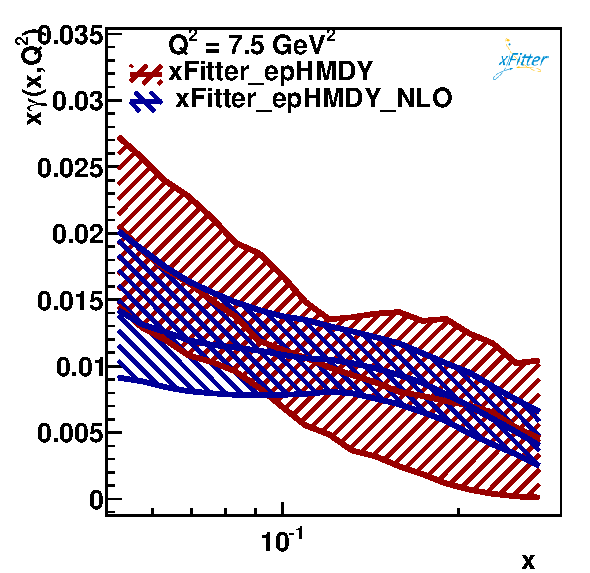
\includegraphics[width=6.96cm]{picture_confirmation/photon_7_5}} 
%\subfigure[]{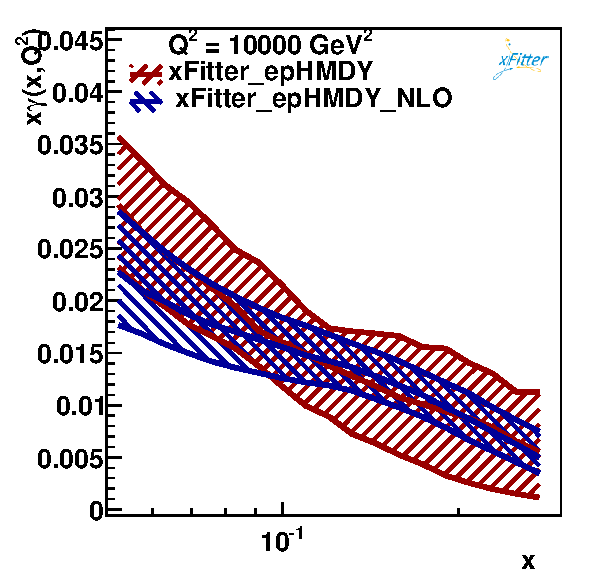
\includegraphics[width=6.96cm]{picture_confirmation/photon_10000}} 
%\caption{Comparison between the photon PDF distributions for the different fits just described above: (a) at the starting scale; (b) at the evolved scale.}
%\label{photon_scan}
%\end{figure}

Fig %Fig.~\ref{photon_zoom} 
shows the photon distribution in the range $0.045 < x < 0.35$, region where high mass DY data are most 
sensitive to this quantity. The new fit results 
have an uncertainty between 20{\%} and 30{\%}, which is 
considerably reduced compared to the  NNPDF30qed NLO photon PDF which is also 
shown for comparison. {\it Not the rwg version}.
The predictions for the LUXqed~\cite{luxqed} photon PDF and the 
HKR photon PDF~\cite{hkr}  are shown compared to the NNLO PDF from the present analysis in Fig.** {\it Compare our NNLO PDF when you have it}.
In this kinematic region, the fit
 predictions agree with LUXqed and with the HKR photon PDF at the 1-$\sigma$ level. 


%\begin{figure}
%\centering
%\subfigure[]{\includegraphics[width=6.96cm]{picture_confirmation/photon_7_5_zoom}} 
%\subfigure[]{\includegraphics[width=6.96cm]{picture_confirmation/photon_10000_zoom}} 
%\caption{Comparison between the photon PDF distributions for the different fits just described above: (a) at the starting scale; (b) at the evolved scale.}
%\label{photon_zoom}
%\end{figure}



%\begin{figure*}[th]
%\begin{centering}
%\includegraphics[width=0.75\textwidth]{figs/}
%\par\end{centering}
%\caption{alphas across bottom transition }
%\end{figure*}

